\section{Model Version Evaluation and Comparison}
Updates to models often lead to superior performance; however, this may come with a detriment to fairness and bias. In this section we want to see how much the version updates in models will be robust toward fairness constraints and errors defined in the previous section. Thus, we will first define this source of bias. Then we will show the results for the models from the previous section that have various versions.  
\begin{figure*}[!bt]
% \includegraphics[width=\textwidth,height=0.9\textwidth,trim=0.5cm 0.2cm 0.4cm 0cm,clip=true]{results1.pdf}
%\begin{subfigure}[b]{\textwidth}
%\centering
% \includegraphics[width=1\textwidth,height=0.16\textwidth,trim=0cm 0cm 0cm 0cm,clip=true]{weighted_combined.pdf}
\begin{subfigure}[b]{0.33\textwidth}
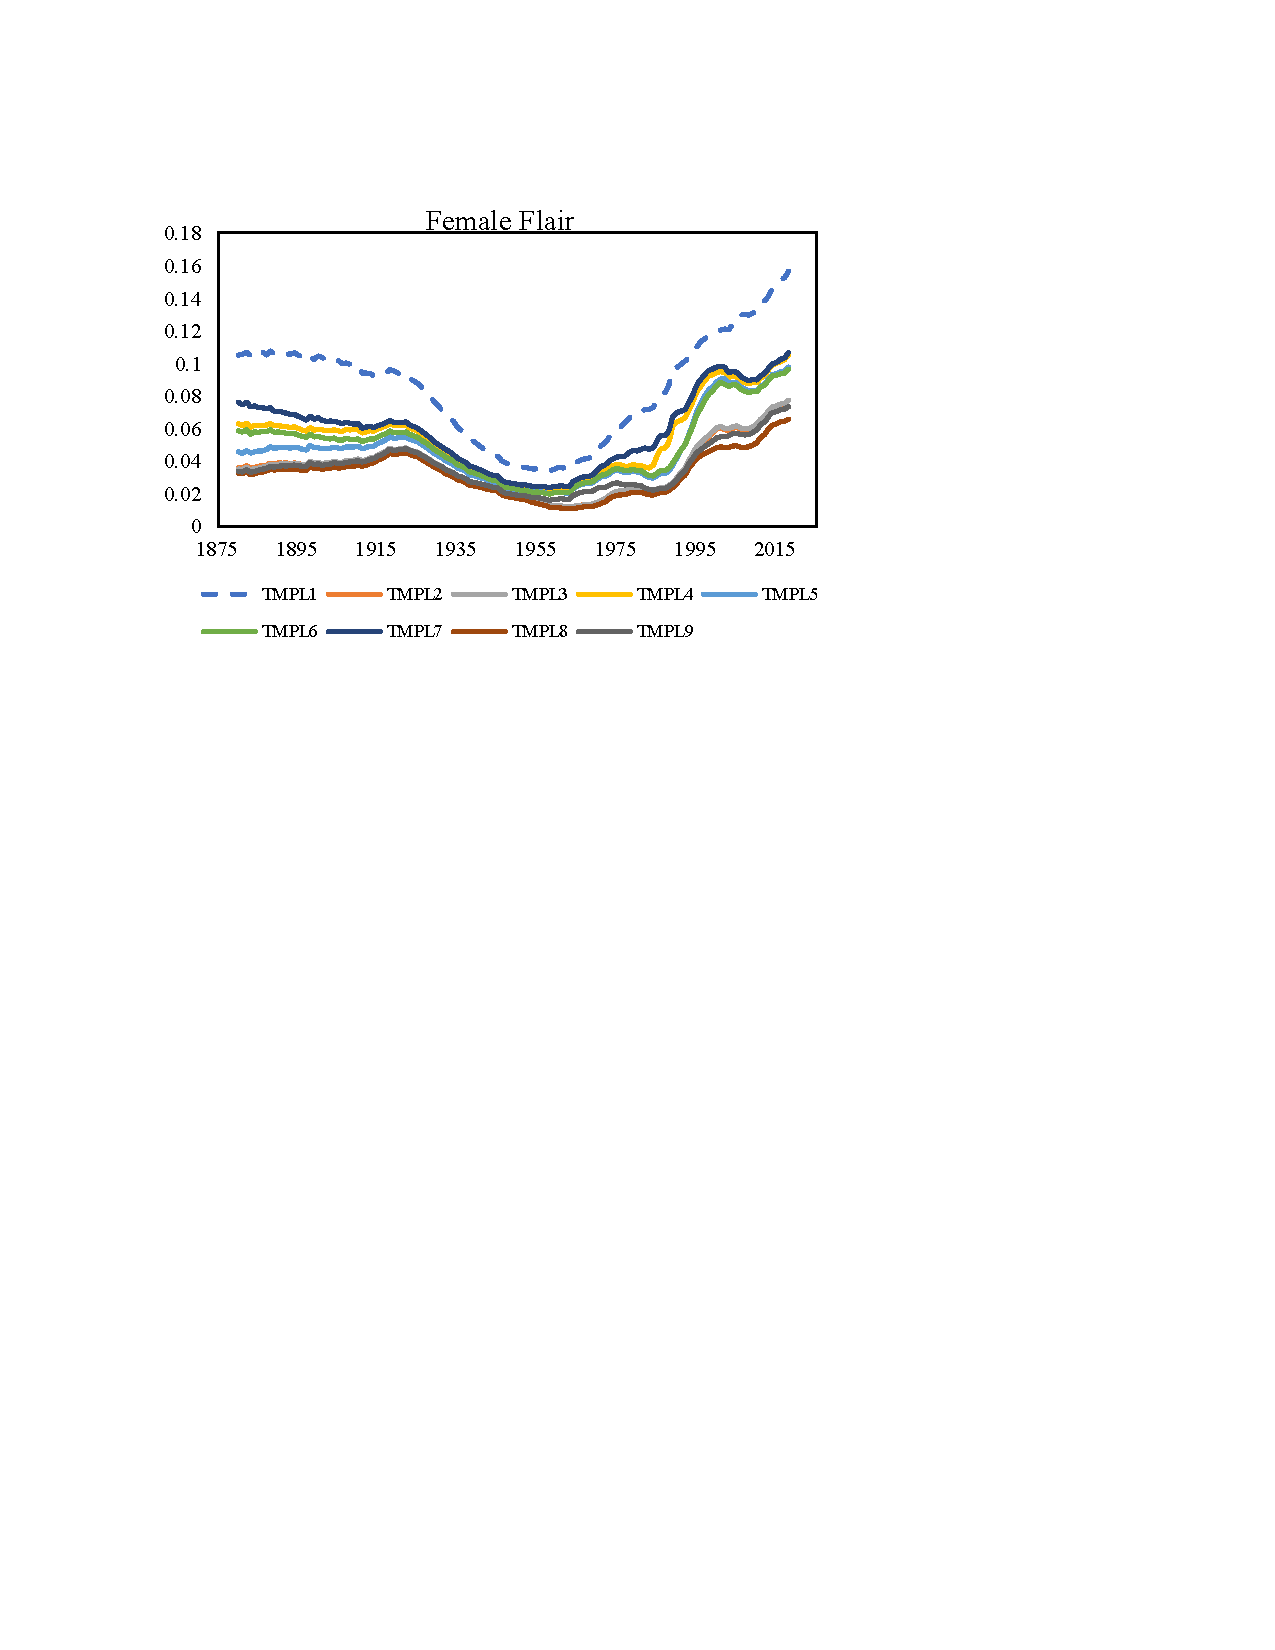
\includegraphics[width=\textwidth,height=0.65\textwidth,trim=0cm 0cm 0cm 0cm,clip=true]{images/template_results/female_flair.pdf}
\end{subfigure}
\begin{subfigure}[b]{0.33\textwidth}
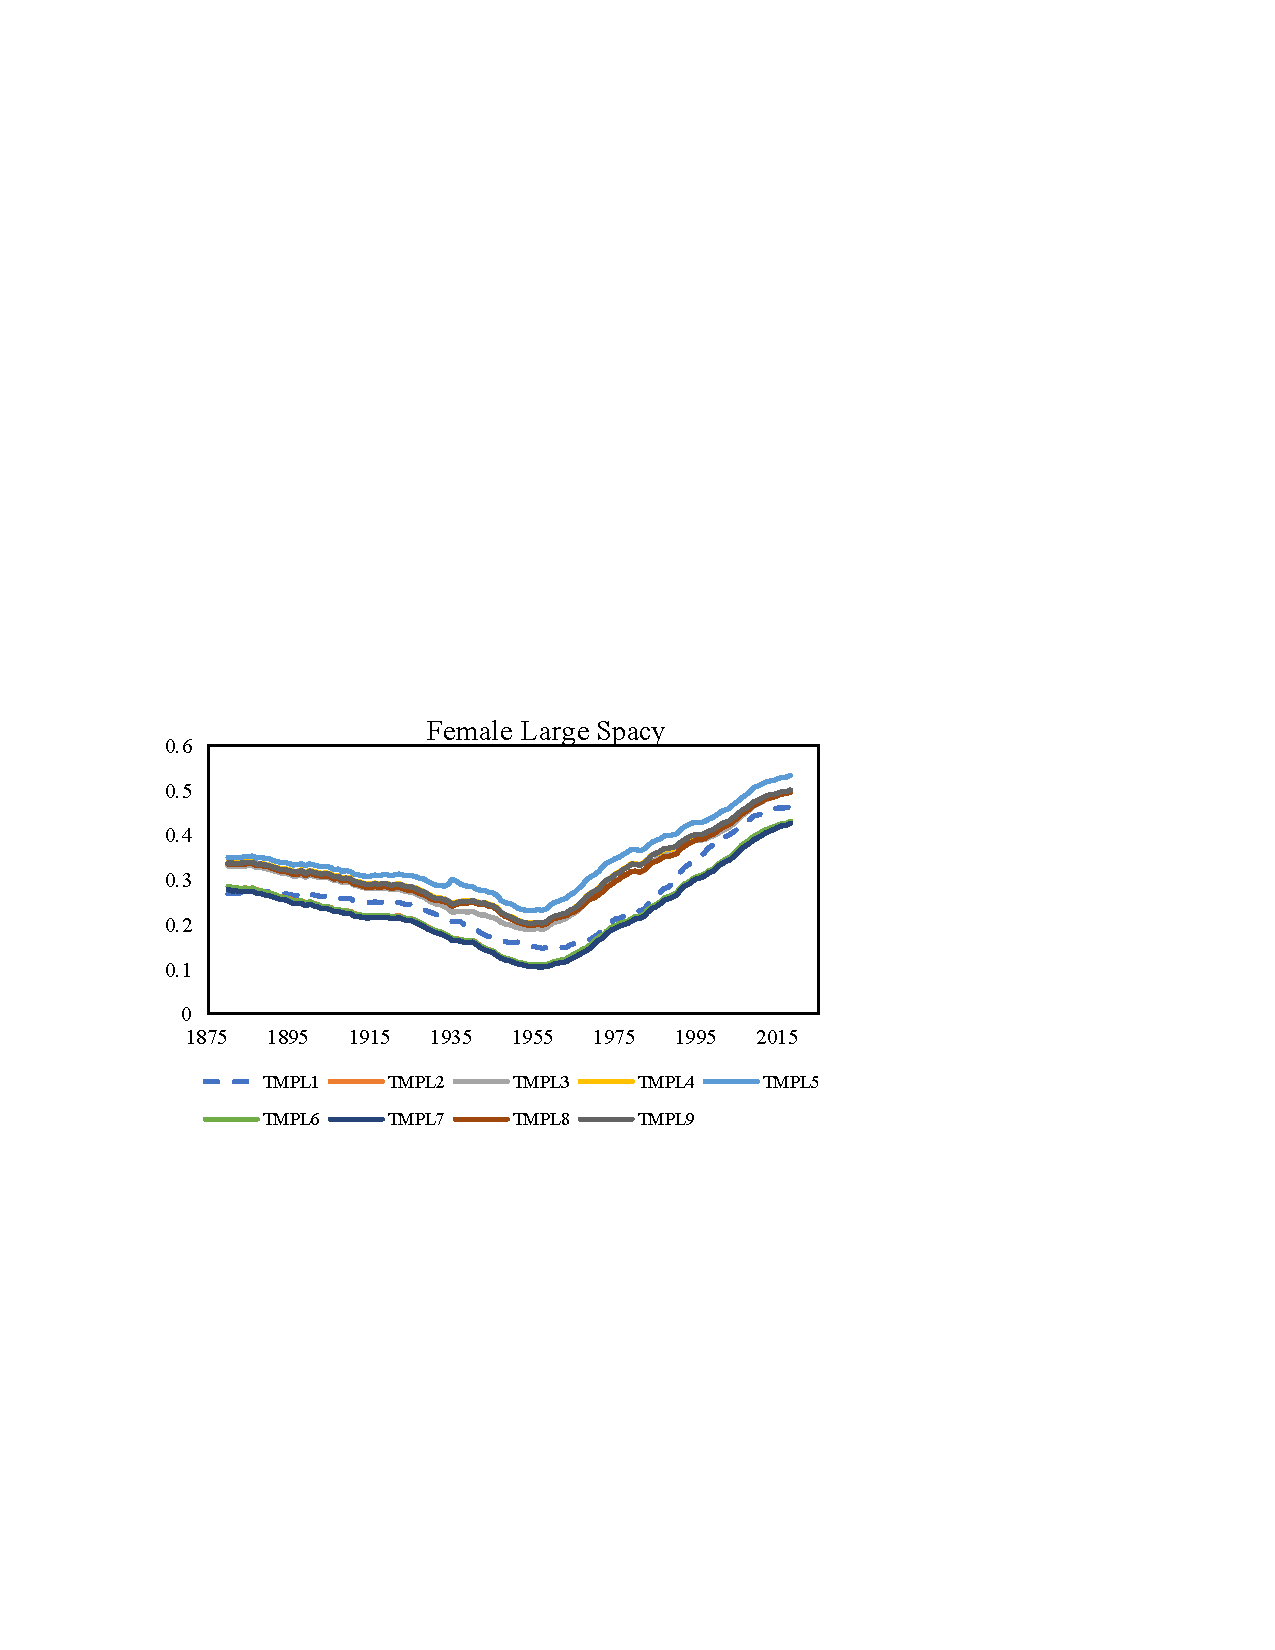
\includegraphics[width=\textwidth,height=0.65\textwidth,trim=0cm 0cm 0cm 0cm,clip=true]{images/template_results/female_spacy.pdf}
\end{subfigure}
\begin{subfigure}[b]{0.33\textwidth}
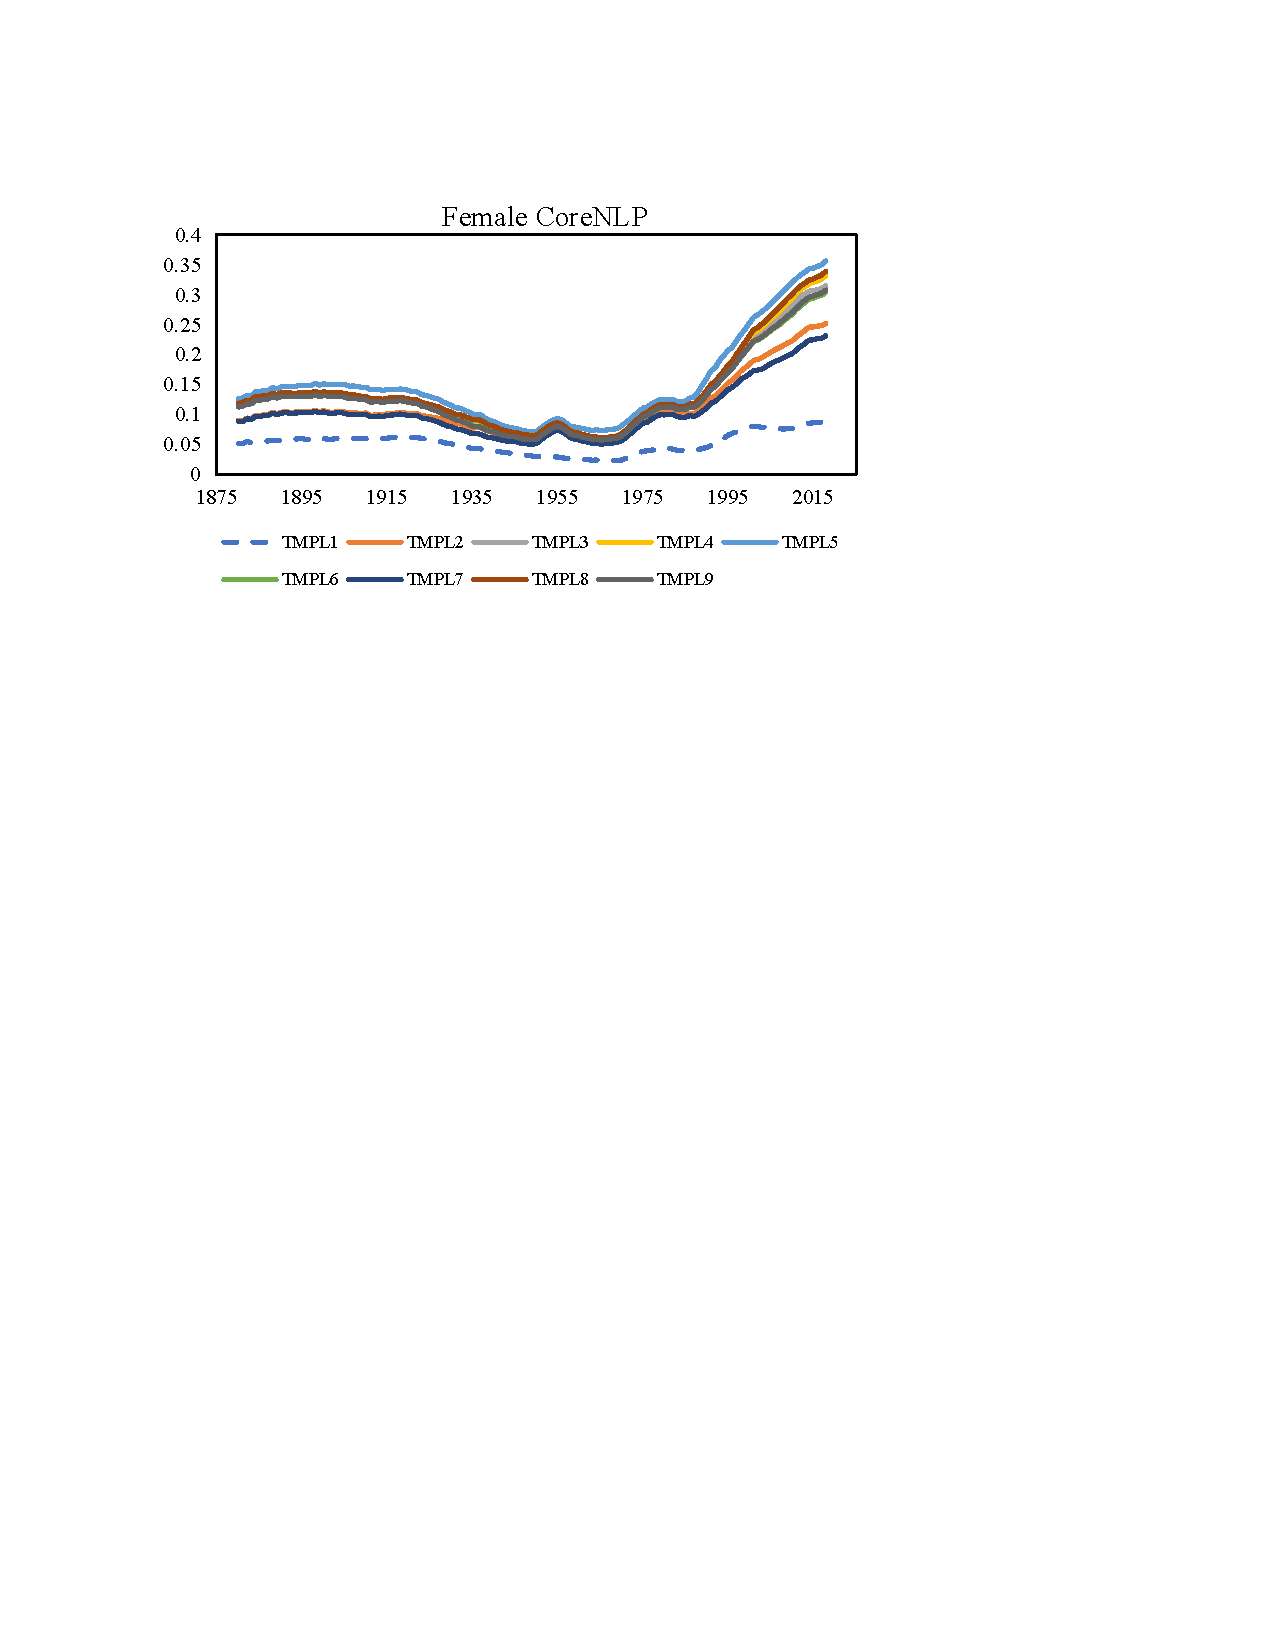
\includegraphics[width=\textwidth,height=0.65\textwidth,trim=0cm 0cm 0cm 0cm,clip=true]{images/template_results/female_corenlp.pdf}
\end{subfigure}
\begin{subfigure}[b]{0.33\textwidth}
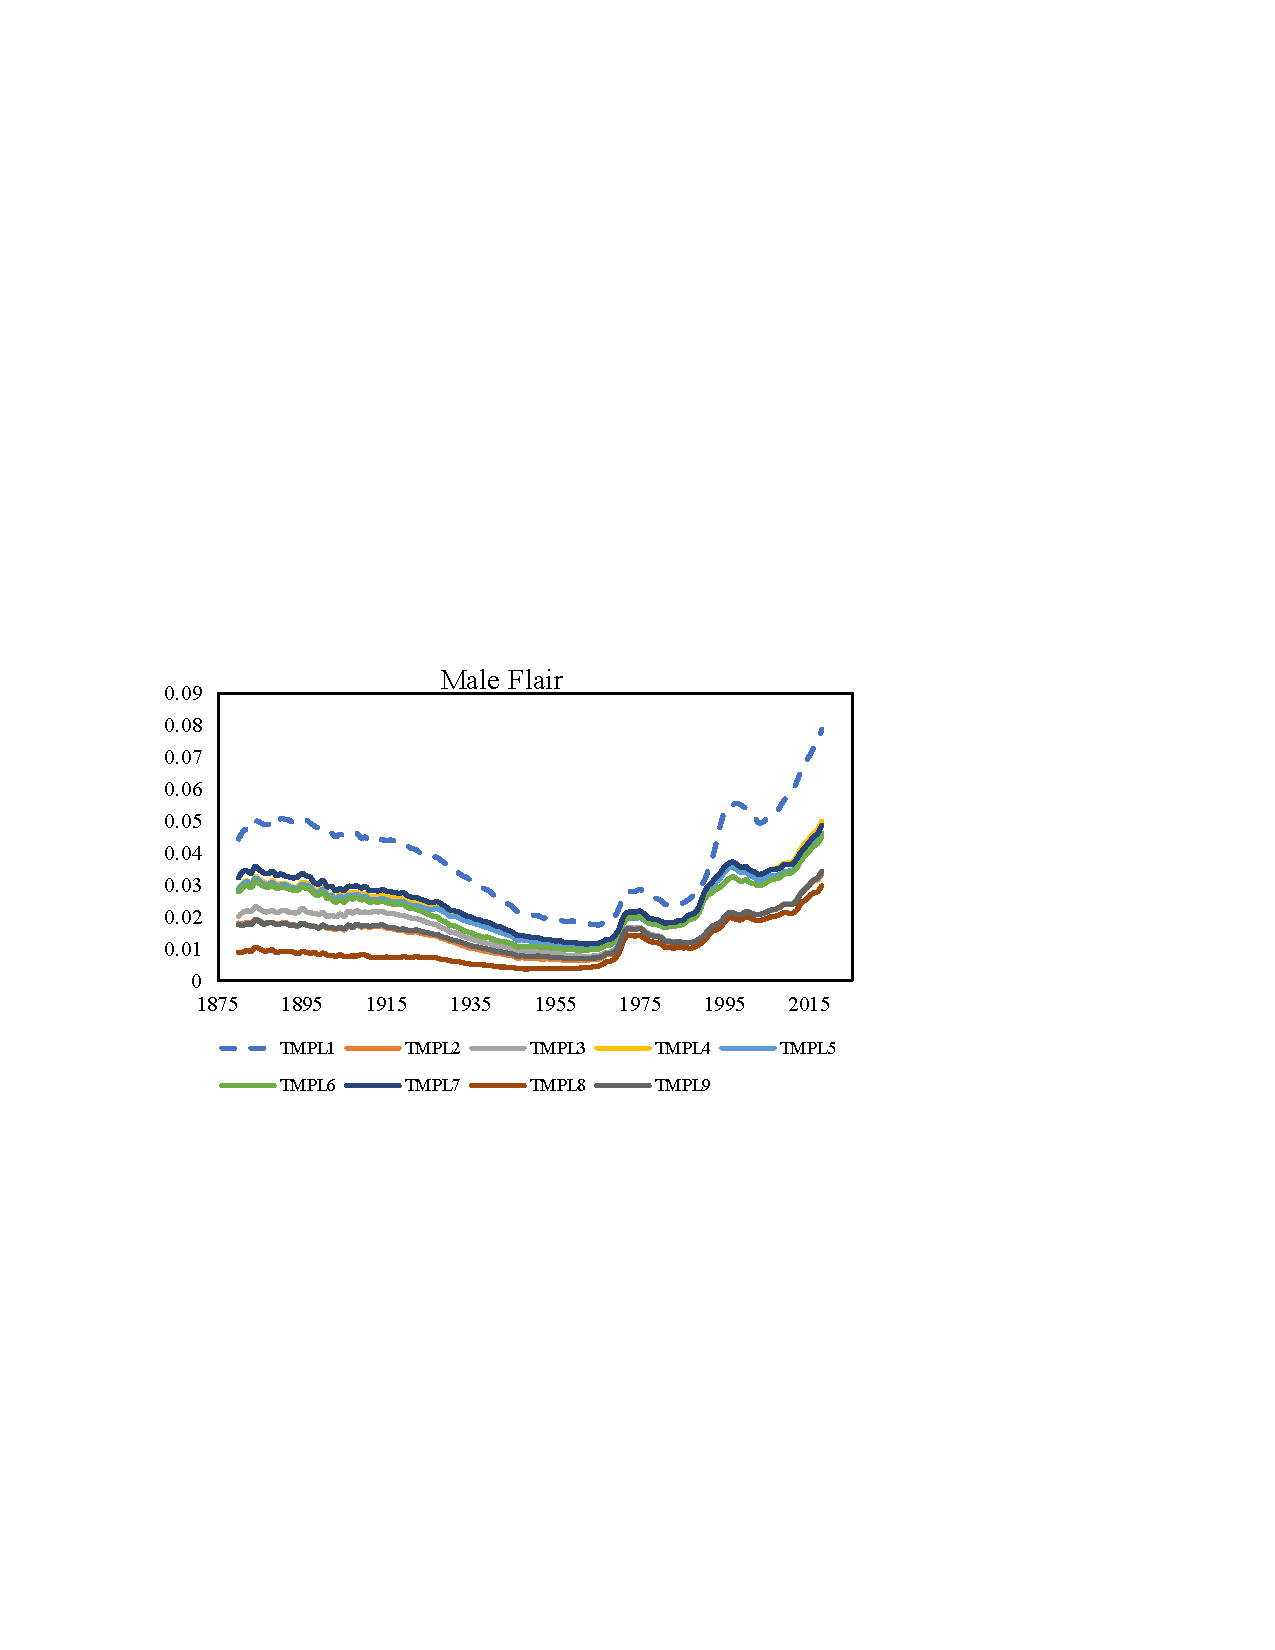
\includegraphics[width=\textwidth,height=0.65\textwidth,trim=0cm 0cm 0cm 0cm,clip=true]{images/template_results/male_flair.pdf}
\end{subfigure}
\begin{subfigure}[b]{0.33\textwidth}
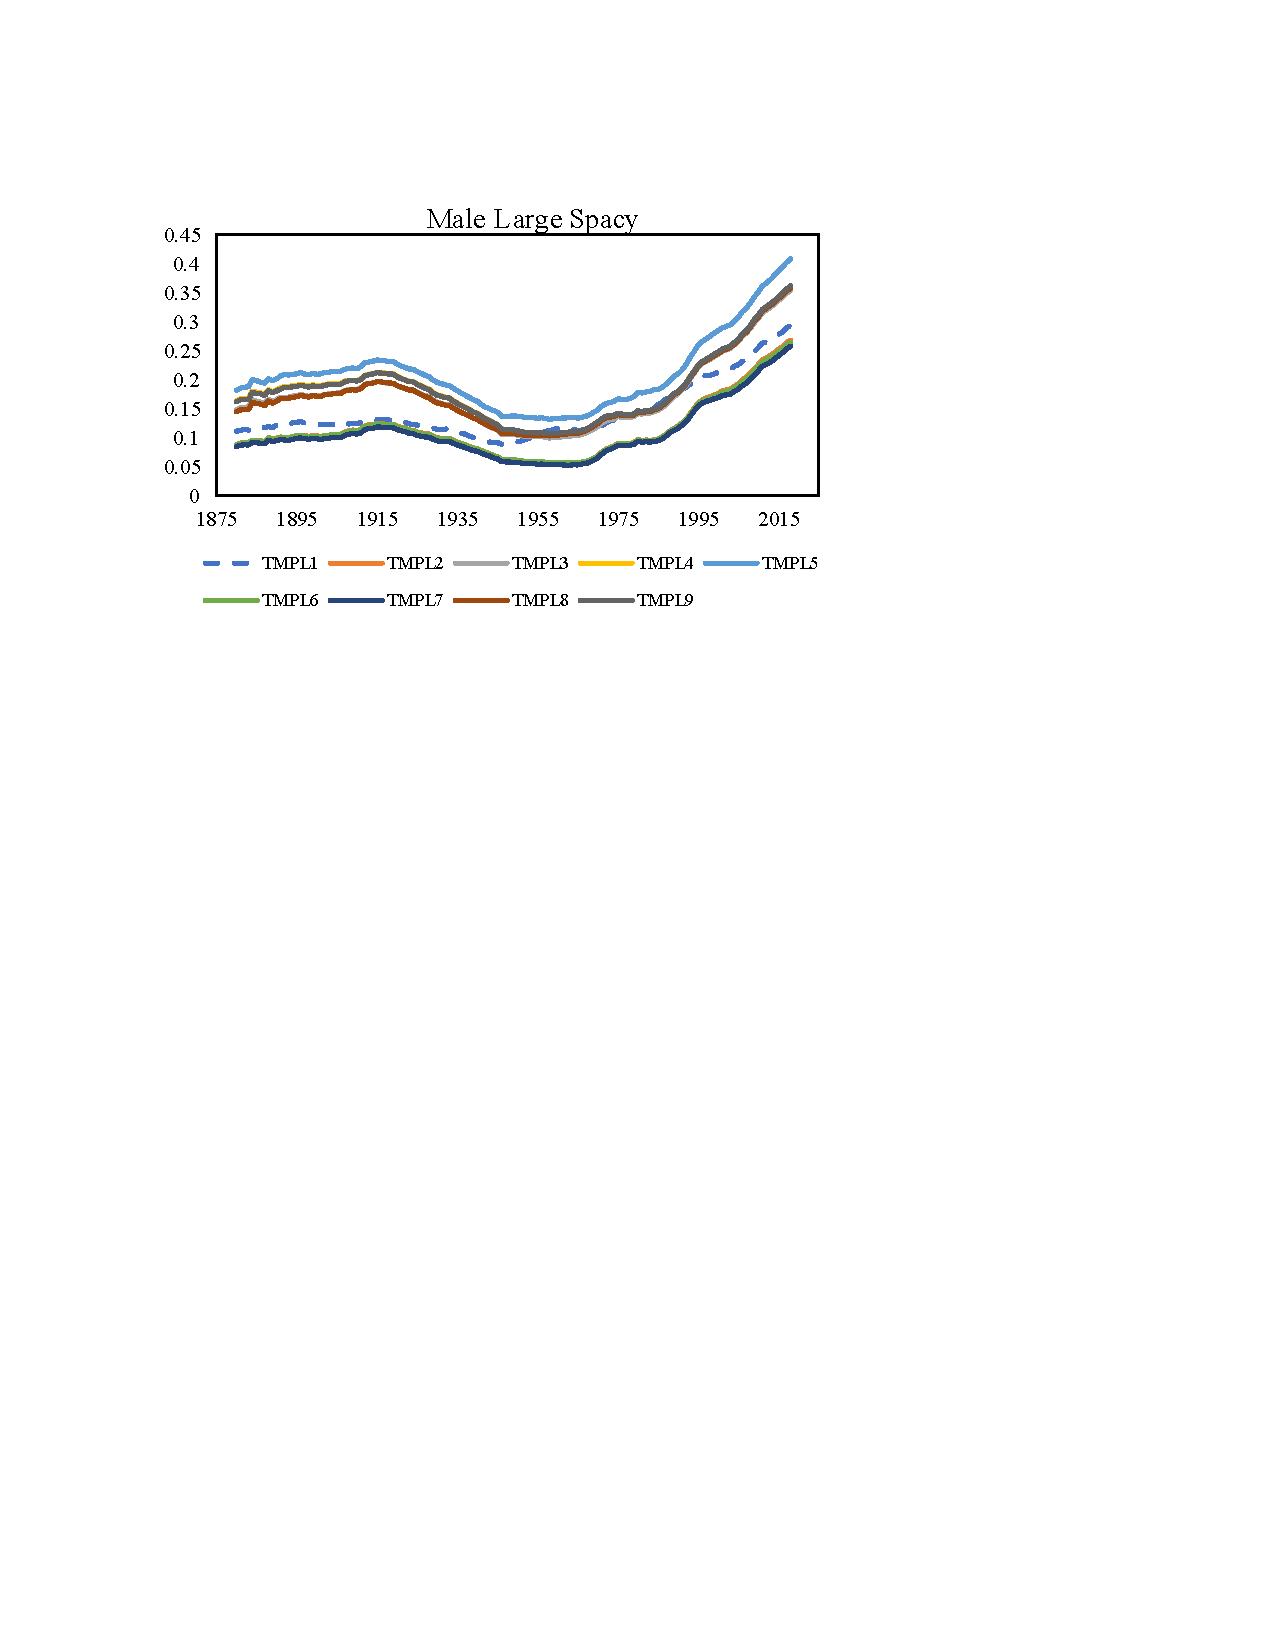
\includegraphics[width=\textwidth,height=0.65\textwidth,trim=0cm 0cm 0cm 0cm,clip=true]{images/template_results/male_spacy.pdf}
\end{subfigure}
\begin{subfigure}[b]{0.33\textwidth}
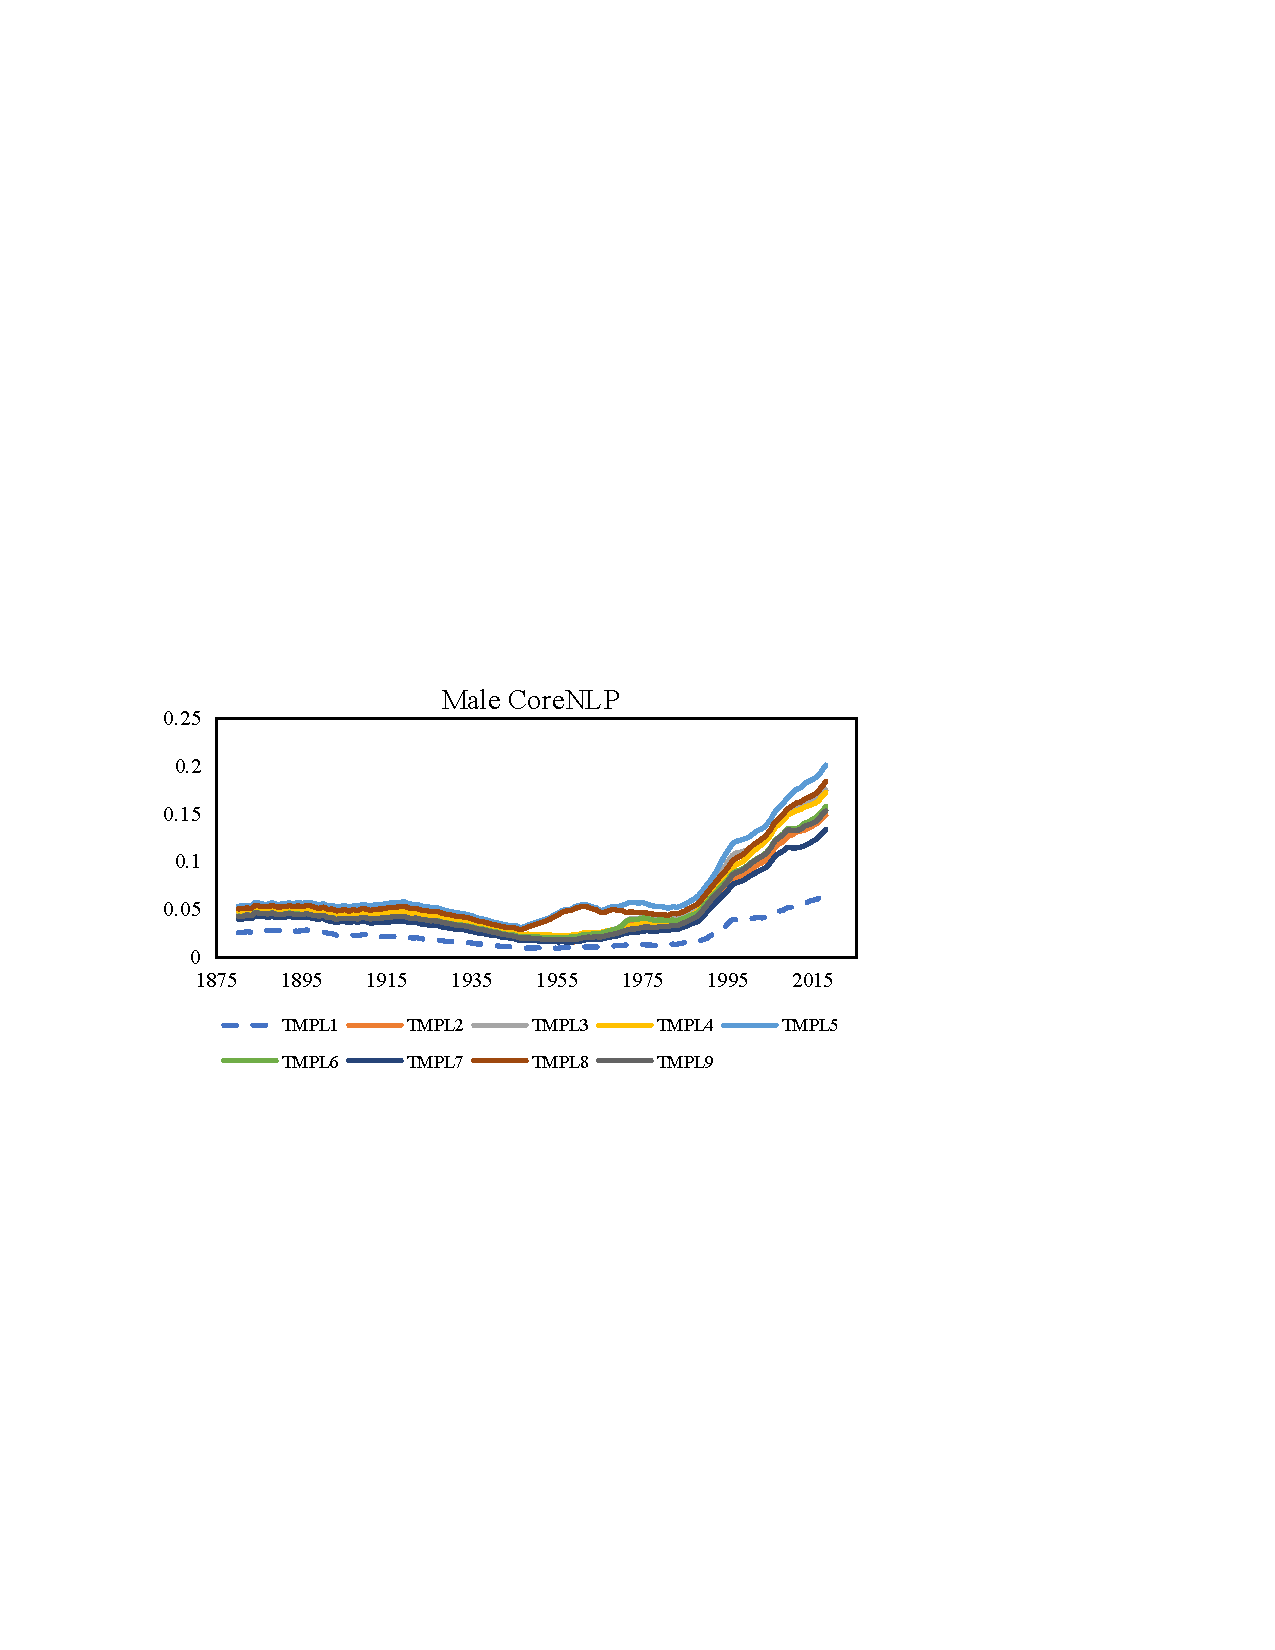
\includegraphics[width=\textwidth,height=0.65\textwidth,trim=0cm 0cm 0cm 0cm,clip=true]{images/template_results/male_corenlp.pdf}
\end{subfigure}
\caption{Performance of different models on different templates from our benchmark for female and male names collected for over 139 years. Notice how context in some of the templates helped some models, but showed negative effects on other models.}
\label{tempresults}
\end{figure*}
\\
\textbf{Definition} \textit{(Version Bias). This is a type of bias that  arises from updates in the systems.}

In order to report the results of our analysis, we used four of our models mentioned in the previous section that have version updates---namely small, medium, and large models from Spacy (versions 2.0 and 2.1) and versions 3.8 and 3.9 from CoreNLP. We then repeated the experiments from the previous section to report the results for Error Type-1, 2, and 3 (Weighted and Unweighted) cases using template \#4 from our benchmark. The results for Spacy show that although in not all cases were updated versions worse than that of the previous versions, there were some cases where  version updates had serious fairness-related issues. For instance, as shown in Figure \ref{spacyv} for the Spacy medium model, the newer version is more erroneous when it comes to the Error Type-1 Weighted case which is a superset of all the error types discussed in this paper. Not only that, the average increase rate of this error is twice that of female names as opposed to male names when updating the model version. These newer versions may try to boost their performance by trying to tag more entities, which indeed would boost their performance when having other non-PERSON entities in the test set. However, these newer tags may be tagging PERSON entities in the relevant context to the non-PERSON counterpart, which is not desirable when evaluated on our benchmark. The reason that we separated the types of errors and created the benchmark is to show the fine-grained and sensitive issues in these systems. Similarly, for CoreNLP more entities tried to be tagged---which resulted in a slight improvement in Error Type-3, as shown in Figure \ref{corenlp_versions}. However, these tags would not correctly assign PERSON tags to PERSON entities, which resulted in a  degraded performance in Error Type-2, as shown in Figure \ref{corenlp_versions} and 
resulted in no change in the overall performance based on Error Type-1 in the newer version update of the CoreNLP model. The results were identical for the unweighted case, and we can see how that degrade in performance was more severe for female names on average. As examples, some of the changes from version 3.8 to version 3.9 of the CoreNLP model are shown in Table \ref{corenlp_version_examples}. 

